% Kompilieren mit: pdflatex -shell-escape uebung
\documentclass{uebblatt}

\begin{document}

\maketitle{1}{Learn You a Haskell for Great Good!}


\section{Aufwärmübungen in GHCi}

\begin{aufgabe}{Verschachtelte Tupel}
Benutze die vordefinierten Funktionen \haskellinline{fst :: (a, b) -> a} und \haskellinline{snd :: (a, b) -> b}, um das Textzeichen aus \haskellinline{(1, ('a', "foo"))} zu extrahieren.
\end{aufgabe}

\begin{aufgabe}{Medianbestimmung}
Sei \haskellinline{xs} eine unsortierte Liste von Zahlen, z.\,B. \haskellinline{let xs = [3, 7, -10, 277, 89, 13, 22, -100, 1]}. Schreibe einen Ausdruck, der den Median (das mittlere Element in einer Sortierung der Liste) von \haskellinline{xs} berechnet. Verwende dazu die Funktion \haskellinline{Data.List.sort}, \haskellinline{length}, \haskellinline{div} und \haskellinline{!!}.
\end{aufgabe}

\begin{aufgabe}{Der Smiley-Operator erster Ordnung}
Was könnte der Ausdruck \haskellinline{(.) . (.)} bewirken? Finde es heraus mit Hilfe von GHCi!
\end{aufgabe}


\section{Spiel und Spaß mit Listenfunktionen}

\begin{aufgabe}{Groß- und Kleinschreibung}
  \begin{enumerate}
    \item Verwende \haskellinline{map}, um einen String in eine Liste von Bools zu verwandeln, die angeben, ob das entsprechende Zeichen im String ein Groß- oder Kleinbuchstabe war.
    Beispielsweise soll bei \haskellinline{"aBCde"} das Ergebnis \haskellinline{[True,False,False,True,True]} sein. \\
    {\scriptsize \emph{Hinweis.} Verwende \haskellinline[fontsize=\scriptsize]{isLower :: Char -> Bool} aus \textinline[fontsize=\scriptsize]{Data.Char}.\par}
    \item Schreibe eine Funktion, die für einen String zurückgibt, ob er nur Kleinbuchstaben enthält.
    \item Berechne die Anzahl der Kleinbuchstaben in einem gegebenen String.
  \end{enumerate}
\end{aufgabe}

\begin{aufgabe}{Typfehler}
  Erkläre den Typfehler, der bei folgendem Ausdruck entsteht: \haskellinline{\x -> x x}
\end{aufgabe}


\section{Funktionsdefinitionen}

\begin{aufgabe}{Fizz buzz}
  Beim Spiel \emph{Fizz buzz} stehen alle Spieler im Kreis. Reihum wird nun von eins hoch gezählt. Anstatt von Zahlen, die durch drei teilbar sind, muss man jedoch "`fizz"' sagen und "`buzz"' bei Zahlen, die durch fünf teilbar sind. Ist eine Zahl sowohl durch drei als auch durch fünf teilbar, so sagt man "`fizz buzz"'. Wer einen Fehler macht, scheidet aus.
  
  Implementiere die unendliche Liste
  \begin{haskellcode}
fizzbuzz :: [String]
fizzbuzz = [ "1", "2", "fizz", "4", "buzz", "fizz", "7", "8", "fizz", "buzz"
           , "11", "fizz", "13", "14", "fizz buzz", "16", ...]
  \end{haskellcode}
\end{aufgabe}

\begin{aufgabe}{Origami}
  Implementiere eine Funktion \haskellinline{maximum' :: [Int] -> Int}, die die größte Zahl in einer Liste zurückliefert oder~\haskellinline{0}, falls die Liste leer ist oder alle Zahlen negativ sind. Verwende dazu \haskellinline{foldl :: (b -> a -> b) -> b -> [a] -> b}.
\end{aufgabe}

\begin{aufgabe}{Fibonacci-Zahlen}
  Die Fibonacci-Folge $0, 1, 1, 2, 3, 5, 8, \ldots$ ist bekanntermaßen rekursiv definiert durch:
  \begin{center}
    \emph{Die nullte Fibonacci-Zahl ist null, die erste Fibonacci-Zahl ist eins, \\
    jede weitere Fibonacci-Zahl ist die Summe ihrer beiden Vorgänger.}
  \end{center}
  \begin{enumerate}
    \item Verwende diese Definition direkt, um eine Haskell-Funktion \haskellinline{fib :: Int -> Int} zu schreiben, die die $n$-te Fibonacci-Zahl berechnet.
    \item Berechne \haskellinline{fib 35}. Was ist das Problem?
    \item Implementiere \haskellinline{fibs :: [Int]}, eine unendliche Liste aller Fibonacci-Zahlen. Lass dir mit \haskellinline{take 100 fibs} die ersten hundert Folgeglieder in GHCi ausgeben. \\
    {\scriptsize \emph{Hinweis.} Du bekommst massig Bonuspunkte, wenn du \haskellinline[fontsize=\scriptsize]{zipWith} verwendest.\par}
  \end{enumerate}
\end{aufgabe}

\begin{aufgabe}{Die Collatz-Vermutung}
  % von https://de.wikipedia.org/wiki/Collatz-Problem
  \begin{itemize}
    \item Beginne mit irgendeiner natürlichen Zahl $n > 0$.
    \item Ist n gerade, so nimm als Nächstes $\tfrac{n}{2}$,
    \item Ist n ungerade, so nimm als Nächstes $3n + 1$.
    \item Wiederhole die Vorgehensweise mit der erhaltenen Zahl.
  \end{itemize}
  Zum Beispiel erhält man für $n=19$ die Folge
  \[ 19, 58, 29, 88, 44, 22, 11, 34, 17, 52, 26, 13, 40, 20, 10, 5, 16, 8, 4, 2, 1, 4, 2, 1, 4, 2, 1, \ldots \]
  \begin{enumerate}
    
    \item Schreibe eine Funktion \haskellinline{collNext :: Int -> Int}, welche Collatz-Iteration durchführt.
    \item Implementiere die Funktion \haskellinline{collSeq :: Int -> [Int]}, die die Folge der Collatz-Iterierten berechnet: \haskellinline{collSeq 10 = [10, 5, 16, 8, 4, 2, 1, 4, 2, 1, 4, 2, 1, ...]}
  \end{enumerate}
  Die bisher ungelöste Collatz-Vermutung besagt, dass man ausgehend von jeder beliebigen Zahl $n$ irgendwann bei $1$ landet.
  \begin{enumerate}
    \setcounter{enumi}{2}
    \item Schreibe die Funktion \haskellinline{collTest :: Int -> Bool}, welche die Collatz-Vermutung für eine Eingabe $n$ testet. Falls die Collatz-Vermutung für $n$ falsch sein sollte, so muss die Funktion nicht terminieren.
    \item Überprüfe die Collatz-Vermutung für alle natürlichen Zahlen kleiner als eine Million.
  \end{enumerate}
\end{aufgabe}

\begin{aufgabe}{Die Prelude}
  Informiere dich, was folgende Funktionen aus der Standardbibliothek tun, und implementiere so viele wie du willst neu:
  \begin{haskellcode}
head, tail, init, last, length, reverse, (++), iterate, map, filter,
intersperse, concat, zipWith, repeat, and, takeWhile, dropWhile, maximum
  \end{haskellcode}
\end{aufgabe}

\begin{aufgabe}{Pointless/pointfree programming}
  Vereinfache folgende Funktionsdefinitionen:
  \begin{haskellcode}
multMany a xs = map (\x -> a*x) xs
filterMap f g xs = filter f (map g xs)
  \end{haskellcode}
\end{aufgabe}

\begin{aufgabe}{Run-Length-Encoding}
  Zur effizienten Speicherung von Daten mit vielen Zeichenwiederholungen bietet es sich an, nicht jedes einzelnes Zeichen, sondern Zeichen mit der jeweiligen Anzahl Wiederholungen zu speichern:
  \begin{haskellcode*}{fontsize=\footnotesize,escapeinside=||}
|\ghci| encode ['a', 'a', 'a', 'a', 'b', 'c', 'c', 'a', 'a', 'd', 'e', 'e', 'e', 'e']
[(4, 'a'), (1, 'b'), (2, 'c'), (2, 'a'), (1, 'd'), (4, 'e')]
  \end{haskellcode*}
  Implementiere die Funktion \haskellinline{encode :: String -> [(Int, Char)]} und die Umkehrfunktion \haskellinline{decode :: [(Int, Char)] -> String}!
\end{aufgabe}

\begin{aufgabe}{Längste Teilfolge}
  Schreibe eine Funktion \haskellinline{longestSubsequence :: (a -> Bool) -> [a] -> [a]}.
  Diese soll die längste zusammenhängende Unterliste in einer Liste berechnen, für die das übergebene Prädikat vom Typ \haskellinline{a -> Bool} den Wert \haskellinline{True} liefert. Wenn beispielsweise \haskellinline{xs :: [Date]} die Liste der letzten 365 Tage ist, und \haskellinline{p :: Date -> Bool} angibt, ob eine gewisse Benutzerin an einem gegebenen Tag auf GitHub aktiv war, so berechnet \haskellinline{longestSubsequence xs p} die längste Strähne auf GitHub.
\end{aufgabe}

\begin{aufgabe}{Kettenbrüche}
  Jede reelle Zahl $r \in \R$ kann als \emph{unendlicher Kettenbruch}
  \[ r = b_0 + \frac{1}{b_1 + \frac{1}{b_2 + \frac{1}{b_3 + \tfrac{1}{\ddots}}}} \]
  mit $b_0 \in \Z$ und $b_i \in \N$, $i \geq 1$ geschrieben werden. Überlege dir einen Algorithmus, der die unendliche Folge der $b_i$'s berechnet und implementiere ihn in Haskell. Überprüfe deinen Algorithmus anhand der Kettenbruchentwicklung von $\pi$ (in Haskell: \haskellinline{pi}). \\
  {\scriptsize \emph{Hinweis.} Du wirst die Funktionen \haskellinline[fontsize=\scriptsize]{floor :: Double -> Int} und \haskellinline[fontsize=\scriptsize]{fromIntegral :: Int -> Double} brauchen.\par}
\end{aufgabe}

\begin{aufgabe}{Türme von Hanoi}
  \begin{minipage}[m]{0.67 \linewidth}
    Die Aufgabe bei Hanoi ist es, einen Turm von Scheiben von einem Steckplatz zu einem anderen zu transportieren. Dabei darf man nur je eine Scheibe einzeln bewegen und es darf niemals eine größere Scheibe auf einer kleineren liegen. Man hat einen Steckplatz als Zwischenlager zur Verfügung.
    Implementiere eine Funktion \haskellinline{toh :: Int -> [(Int, Int)]}, welche die Hanoi-Züge (Bewegungen von einzelnen) berechnet, mit denen man einen Turm einer gewissen Größe von Steckplatz $1$ zu Steckplatz $3$ mit Steckplatz $2$ als Zwischenlager bewegen kann.
  \end{minipage}
  \begin{minipage}{0.32 \linewidth}
    \hfill 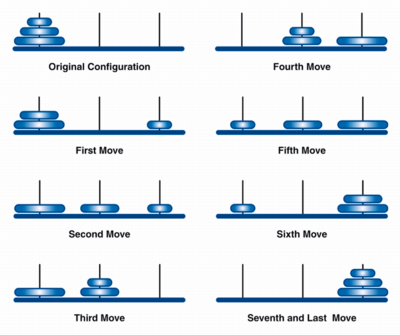
\includegraphics[width=5cm]{towers-hanoi.png}
  \end{minipage}
  
  \begin{haskellcode*}{fontsize=\small,escapeinside=||}
|\ghci| toh 3
[(1,3), (1,2), (3,2), (1,3), (2,1), (2,3), (1,3)]
  \end{haskellcode*}
  
  {\scriptsize \emph{Tipp.} Definiere eine Hilfsfunktion \haskellinline[fontsize=\scriptsize]{moveTower :: Int -> (Int, Int, Int) -> [(Int, Int)]}, sodass \haskellinline[fontsize=\scriptsize]{moveTower n (x, y, z)} die nötigen Schritte ausgibt, um $n$ Scheiben von $x$ nach $y$ unter Verwendung von $z$ als Zwischenlager zu bewegen.\par}
\end{aufgabe}


\section{Eigene Datentypen}

\begin{aufgabe}{Binäre Bäume}
Im Folgenden verwenden wir folgende Definition für binäre Bäume, deren
Verzweigungsknoten mit Werten vom Typ~\haskellinline{Int} dekoriert sind.
\begin{haskellcode}
data Tree = Nil | Fork Int Tree Tree
    deriving (Show)
\end{haskellcode}
\begin{enumerate}
\item Schreibe eine Funktion, die die Gesamtzahl Blätter eines Baums berechnet: \\
\haskellinline{numberOfLeaves :: Tree -> Int}.
\item Schreibe eine Funktion, die die Höchsttiefe eines Baums berechnet.
\item Schreibe eine Funktion, die die Int-Werte der Verzweigungsknoten in einer
Reihenfolge deiner Wahl als Liste zurückgibt.
\end{enumerate}
\end{aufgabe}

\begin{aufgabe}{Binäre Bäume bilden einen Funktor}
\begin{enumerate}
\item Verallgemeinere die vorherige Aufgaben auf Bäume, die Werte von
einem beliebigen Typ~\haskellinline{a} statt~\haskellinline{Int} tragen.
Vervollständige dazu zunächst folgende Definition:
\begin{haskellcode}
data Tree a = Nil | ...
    deriving (Show)
\end{haskellcode}
\item Implementiere eine Funktion \haskellinline{tmap :: (a -> b) -> Tree a ->
Tree b}.
\end{enumerate}
\end{aufgabe}

\begin{aufgabe}{Unendliche Bäume}
\begin{enumerate}
\item Schreibe eine Funktion \haskellinline{cutOff :: Int -> Tree a -> Tree a}, die eine
Maximaltiefe und einen Baum als Argumente nimmt und einen neuen Baum
zurückgibt, der sich aus dem gegebenen durch Abschneidung bei der gegebenen
Maximaltiefe ergibt.
\item Definiere eine Funktion, die eine unendliche Liste von Werten nimmt und
einen Baum zurückgibt, auf dessen Verzweigungsknoten die Elemente der Liste
sitzen. Suche dir selbst aus, in welcher Reihenfolge die Listenelemente auf dem
Baum platziert werden sollen.
\end{enumerate}
\end{aufgabe}

\begin{aufgabe}{Der Stern--Brocot-Baum (für Fans von Kettenbrüchen)}
Informiere dich auf Wikipedia über den Stern--Brocot-Baum und implementiere ein
Haskell-Programm, dass diesen unendlichen Baum berechnet. Hole dir
gegebenenfalls einen (stark spoilernden) Tipp ab.
\end{aufgabe}

\begin{aufgabe}{Termbäume}
\begin{enumerate}
\item Implementiere einen Datentyp für Funktionsterme. Zum Beispiel soll
\[ (x \cdot x + 3) - x \]
so repräsentiert werden: \haskellinline{Sub (Add (Mul Var Var) (Lit 3)) Var}.
\item Schreibe eine Funktion \haskellinline{eval :: Exp -> Double -> Double},
die in einem gegebenen Term für die Variable~$x$ einen konkreten Wert einsetzt.
\item Schreibe eine Funktion \haskellinline{diff :: Exp -> Exp}, die
einen gegebenen Funktionsterm ableitet. Zum Beispiel soll \haskellinline{diff
(Mul Var Var)} im Wesentlichen äquivalent sein zu \haskellinline{Mul (Lit 2) Var}.
\end{enumerate}
\end{aufgabe}

\begin{aufgabe}{Isomorphe Typen}
Manche Typen lassen sich verlustfrei ineinander umwandeln, zum Beispiel die
folgenden beiden:
\begin{haskellcode}
data Bool    = False  | True  -- schon vordefiniert
data Aussage = Falsch | Wahr
\end{haskellcode}
Man spricht in einem solchen Fall von \emph{zueinander isomorphen Typen}. Die
Umwandlungsfunktionen heißen \emph{Isomorphismen} und können in diesem Fall wie
folgt definiert werden:
\begin{haskellcode}
iso :: Bool -> Aussage
iso False = Falsch
iso True  = Wahr

osi :: Aussage -> Bool
osi Falsch = False
osi Wahr   = True
\end{haskellcode}
Das charakteristische an diesen beiden Funktionen ist, dass~\haskellinline{osi
. iso == id} und~\haskellinline{iso . osi == id}.

Folgende Typen sind jeweils zueinander isomorph. Implementiere
auf analoge Weise Funktionen~\haskellinline{iso} und~\haskellinline{osi}, die
das bezeugen!
\begin{enumerate}
\item \haskellinline{(a, b)}          versus \haskellinline{(b, a)}
\item \haskellinline{((a, b), c)}     versus \haskellinline{(a, (b, c))}
\item \haskellinline{(a, Either b c)} versus \haskellinline{Either (a, b) (a, c)}
\item \haskellinline{a -> (b, c)}     versus \haskellinline{(a -> b, a -> c)}
\item \haskellinline{(a, b) -> c}     versus \haskellinline{a -> b -> c}
\end{enumerate}
\end{aufgabe}


\section{Typklassen}

\begin{aufgabe}{Eigene Show-Instanzen}
Für Debugging-Zwecke oder auch zum Datenaustausch ist die Show-Klasse nützlich,
deren Definition in etwa die folgende ist:
\begin{haskellcode}
class Show a where
    show :: a -> String
\end{haskellcode}
Bei der Deklaration eines neuen Datentyps hat man die Möglichkeit, mit einer
\haskellinline{deriving}-Klausel den Compiler anzuweisen, automatisch eine
geeignete Show-Instanz zu generieren:
\begin{haskellcode}
data Tree a = Nil | Fork a (Tree a) (Tree a)
    deriving (Show)
\end{haskellcode}
In dieser Aufgabe aber sollst du den dafür nötigen Boilerplate-Code von Hand
schreiben. Such dir einen Datentyp deiner Wahl aus und schreibe eine
individuelle Show-Instanz für ihn.
\end{aufgabe}

\begin{aufgabe}{Die Monoid-Typklasse}
Das Modul \haskellinline{Data.Monoid} definiert die Monoid-Typklasse:
\begin{haskellcode}
class Monoid a where
    mempty  :: a
    mappend :: a -> a -> a
    mconcat :: [a] -> a
\end{haskellcode}
Ihr gehören solche Typen an, die eine sog. \emph{Monoidstruktur} tragen. (Wenn
du diesen Begriff nicht kennst, dann frag kurz nach!) Das neutrale Element soll
durch \haskellinline{mempty} angegeben werden, die Monoidoperation durch
\haskellinline{mappend}. Die Funktion \haskellinline{mconcat} soll gleich
mehrere Elemente miteinander verknüpfen.\footnote{Die Funktionen
\haskellinline{mappend} und \haskellinline{mconcat} lassen sich gegenseitig
ausdrücken. Fällt dir ein Grund ein, wieso trotzdem beide Funktionen Teil der
Klasse sind? Hätte man nicht auch einfach \haskellinline{mconcat} außerhalb der
Klasse definieren können?}

\begin{enumerate}
\item Gebe einer Nachimplementierung des Listen-Datentyps, etwa
\haskellinline{data List a = Nil | Cons a (List a)} eine Monoid-Instanz.
Vergiss nicht, zu Beginn deines Programmtexts mit \haskellinline{import
Data.Monoid} die Definition der Monoid-Klasse zu laden.
\item Implementiere folgende Funktion:
\begin{haskellcode}
cata :: (Monoid m) => (a -> m) -> ([a] -> m)
\end{haskellcode}
\end{enumerate}
\end{aufgabe}

\begin{aufgabe}{Sortierung nach mehreren Kriterien}
Oft steht man vor folgendem Problem: Eine Liste von Dingen soll nach mehreren
Kriterien sortiert werden. Etwa zunächst nach Nachname, unter gleichen
Nachnamen aber nach Vorname und unter gleichem Namen nach Geburtsdatum. Die
in Haskell idiomatische Herangehensweise an dieses Problem verwendet \ldots{}
Monoide!

\begin{enumerate}
\item Schlage den \haskellinline{Ordering}-Typ nach.
\item Reimplementiere die Funktion
\begin{haskellcode}
comparing :: (Ord a) => (b -> a) -> b -> b -> Ordering
\end{haskellcode}
aus dem Modul \haskellinline{Data.Ord}. Sie kann zum Beispiel so verwendet werden:
\begin{haskellcode}
import Data.List

data Person = MkPerson
    { lastName  :: String
    , givenName :: String
    , birthday  :: String
    }
    deriving (Show)

sortPersons :: [Person] -> [Person]
sortPersons = sortBy (comparing lastName)

-- sortBy hat den Typ (a -> a -> Ordering) -> [a] -> [a].
\end{haskellcode}
\item Trägt ein Typ~\haskellinline{a} eine Monoidstruktur, so auch der
Typ~\haskellinline{e -> a} der Funktionen von~\haskellinline{e}
nach~\haskellinline{a}. Bestätige das, indem du folgenden Code vervollständigst:
\begin{haskellcode}
instance (Monoid a) => Monoid (e -> a) where
    -- ...
\end{haskellcode}
Da diese Instanz schon in~\haskellinline{Data.Monoid} vordefiniert ist, musst
du für diese Teilaufgabe den Import von\haskellinline{Data.Monoid} entfernen
und die Monoid-Typklasse selbst definieren.
\item Was macht folgender Code? Wieso tut er das? Informiere dich dazu über
die Monoid-Instanz von \haskellinline{Ordering} und erinnere dich an die
Monoid-Instanz von Funktionstypen.
\begin{haskellcode}
sortBy $ mconcat
    [ comparing lastName
    , comparing firstName
    , comparing birthday
    ]
\end{haskellcode}
\end{enumerate}
\end{aufgabe}

\begin{aufgabe}{Endliche Typen}
Manche Typen fassen nur endlich viele Werte, zum Beispiel~\haskellinline{Bool}
und~\haskellinline{Either Bool Bool}. Für solche Typen ist es gelegentlich
praktisch, eine vollständige Liste ihrer Werte zu kennen. Aus diesem Grund
führen wir folgende Klasse ein:
\begin{haskellcode}
class Finite a where
    elems :: [a]
\end{haskellcode}
\begin{enumerate}
\item Implementiere eine Finite-Instanz für~\haskellinline{Bool}.
\item Implementiere folgende allgemeinen Instanzen:
\begin{haskellcode}
instance (Finite a, Finite b) => Finite (a,b)        where ...
instance (Finite a, Finite b) => Finite (Maybe a)    where ...
instance (Finite a, Finite b) => Finite (Either a b) where ...
\end{haskellcode}
\item Wenn du Lust auf eine Herausforderung hast, dann implementiere auch
folgende Instanz. Sie ist für die weiteren Teilaufgaben aber nicht nötig.
\begin{haskellcode}
instance (Eq a, Finite a, Finite b) => Finite (a -> b) where ...
\end{haskellcode}
\item Implementiere eine Funktion \haskellinline{exhaustiveTest :: (Finite a) =>
(a -> Bool) -> Bool}.
\item Die Gleichheit zweier Funktionen (vom selben Typ) ist im Allgemeinen
nicht entscheidbar, denn zwei Funktionen sind genau dann gleich, wenn sie auf
allen Eingabewerten übereinstimmen. Um das zu überprüfen, muss man im
Allgemeinen unendlich viele Fälle in Augenschein nehmen. Wenn der Quelltyp aber
endlich ist, geht es doch. Implementiere also:
\begin{haskellcode}
instance (Finite a, Eq b) => Eq (a -> b) where ...
\end{haskellcode}
\end{enumerate}
\end{aufgabe}

\begin{aufgabe}{Abzählbare Typen}
Manche Typen sind zwar nicht endlich, aber immer noch \emph{abzählbar}: Das
heißt, dass es eine unendliche Liste gibt, in der alle Werte des Typs
vorkommen. Zum Beispiel ist der Typ~\haskellinline{Integer} abzählbar, denn in
der Liste~\haskellinline{[0, 1, -1, 2, -2, ...]} kommen alle ganzen Zahlen vor.
\begin{enumerate}
\item Definiere nach dem Vorbild der Finite-Typklasse aus der vorherigen
Aufgabe eine Countable-Typklasse.
\item Implementiere eine Countable-Instanz von~\haskellinline{Integer}.
\item Vervollständige folgenden Code:
\begin{haskellcode}
instance (Countable a, Countable b) => Countable (a,b) where ...
\end{haskellcode}
\item Vervollständige folgenden Code (schwierig!):
\begin{haskellcode}
instance (Countable a) => Countable [a] where ...
\end{haskellcode}
Dabei soll~\haskellinline{[a]} für den Typ der endlichen Listen mit Werten
in~\haskellinline{a} stehen -- obwohl der Typ~\haskellinline{[a]} ja auch
unendliche Listen enthält. Solche \emph{sozialen Verträge} sind in Haskell
leider gelegentlich nötig -- man benötigt abhängige Typen und andere
Entwicklungen, um sie vollständig zu vermeiden. Sauberer wäre an dieser Stelle,
einen neuen Datentyp~\haskellinline{FiniteList a} zu definieren, der isomorph
zum gewöhnlichen Listentyp ist, aber den sozialen Vertrag an zentraler Stelle
kundtut.
\end{enumerate}
\end{aufgabe}

\begin{aufgabe}{Überabzählbare Typen}
Diese Aufgabe richtet sich nur an Leute, die das sog. \emph{Cantorsche
Diagonalargument} und die \emph{Russelsche Antinomie} kennen. Sorry! Bei
Gelegenheit suchen wir eine einführende Referenz.

Wir definieren ein Typalias für Mengen:
\begin{haskellcode}
type Set a = a -> Bool
-- Ist `f :: Set a`, so soll `f x == True` bedeuten, dass `x` in
-- der Menge `f` liegt.
\end{haskellcode}
\begin{enumerate}
\item Setze in diesem Modell die leere Menge, die Universalmenge (welche alle
Werte überhaupt enthält) und die Menge, die nur ein bestimmtes Element enthält,
um. Welche Voraussetzung an den Typ~\haskellinline{a} musst du im letzten Teil
stellen?
\item Implementiere folgende Funktionen:
\begin{haskellcode}
member       :: a     -> Set a -> Bool
union        :: Set a -> Set a -> Set a
intersection :: Set a -> Set a -> Set a
complement   :: Set a -> Set a
\end{haskellcode}
\item Setze die Russelsche Antinomie in Haskell um. Definiere also eine Menge
all derjenigen Mengen, die sich nicht selbst enthalten. Wie äußert sich das
paradoxe Verhalten in Haskell?
\item Setze das Cantorsche Diagonalargument in Haskell um. Definiere also eine
Funktion
\begin{haskellcode}
cantor :: (a -> Set a) -> Set a
\end{haskellcode}
die folgendes leistet: Für jede Funktion~\haskellinline{f :: a -> Set a}
soll~\haskellinline{cantor f} eine Menge sein, die nicht im Bild (in der
Wertemenge) von~\haskellinline{f} enthalten ist.
\item Bonusfrage zum Grübeln: Die vorherige Teilaufgabe zeigt, dass es in
Haskell überabzählbare Typen gibt. Andererseits ist die Menge der
Haskell-Programme abzählbar. Wie passt das zusammen?
\item Literatur dazu: ein toller Blog-Post von sigfpe.
\url{http://blog.sigfpe.com/2008/01/type-that-should-not-be.html}
\end{enumerate}
\end{aufgabe}


\section{Die IO-Monade und andere Monaden}

\begin{aufgabe}{IO-Stringmanipulation}
Schreibe ein Programm, das eine Zeichenkette einliest und diese ruckwärts wieder ausgibt. Die Funktion~\haskellinline{reverse :: [a] -> [a]} könnte hilfreich sein, wenn du dir sie nicht selbst schreiben willst.
\end{aufgabe}

\begin{aufgabe}{Überprüfung von Nutzereingaben}
Schreibe ein Programm, das den Benutzer solange nach einer Zahl fragt, bis dieser eine Zahl angibt, die durch~3 teilbar ist. Erinnere dich an die Typklasse \haskellinline{Read}!
\end{aufgabe}

\begin{aufgabe}{Monadische Schleifen}
\begin{enumerate}
\item Schreibe eine Funktion, die eine gegebene IO-Aktion (oder eine andere Art Aktion) eine gewisse Anzahl von Malen wiederholt. Die Typsignatur sollte also \haskellinline{replicateM :: Int -> [IO a] -> IO [a]} (oder allgemeiner \haskellinline{replicateM :: (Monad m) => Int -> [m a] -> m [a]} -- erinnere dich, dass \haskellinline{IO} eine Instanz von \haskellinline{Monad} ist!) sein.
\item Schreibe eine Funktion \haskellinline{forM :: (Monad m) => [a] -> (a -> m b) -> m [b]} die das tut, was ihr Name und ihre Typsignatur versprechen.
\item Schreibe eine Funktion, die es erlaubt, eine IO-Aktion (oder eine andere Art Aktion) unendlich oft zu wiederholen. Die Typsignatur sollte \haskellinline{forever :: (Monad m) => m a -> m b} sein. Erinnere dich, dass \haskellinline{IO} eine Instanz von \haskellinline{Monad} ist!
\end{enumerate}
\end{aufgabe}

\begin{aufgabe}{Zahlenratespiel}
Schreibe ein Programm, das versucht eine Zahl zwischen 0 und 100 zu erraten, die sich die Nutzerin oder der Nutzer ausgedacht hat. Der Nutzende soll jeweils bei jedem Rateversuch angeben, ob die geratene Zahl kleiner oder größer als die tatsächliche ist. Du kannst das Problem mit einer binären Suche lösen.
\end{aufgabe}

\begin{aufgabe}{Die Reader-Monade}
Gelegentlich muss ein bestimmter Werte durch viele Funktionen gefädelt werden,
zum Beispiel ein Wert, der globale Konfigurationsoptionen enthält:
\begin{haskellcode}
f :: Config -> Int -> Char -> Bool -> Mumble
f config x y z = ...g config x......h config y......z...

g :: Config -> Int -> Gabambel
g config x     = ...x...

h :: Config -> Char -> Rainbow
h config y     = ...p config y......y...

p :: Config -> Char -> Lollipop
p config y     = ...y...
\end{haskellcode}
Vielleicht findest du das nervig. Informiere dich über die Reader-Monade, mit
der man das vermeiden kann. Die neuen Typsignaturen lauten dann:
\begin{haskellcode}
f :: Int -> Char -> Bool -> Reader Config Mumble
g :: Int -> Reader Config Gabambel
h :: Char -> Reader Config Rainbow
p :: Char -> Reader Config Lollipop
\end{haskellcode}
Durch Verwendung von Typsynonymen, wie~\haskellinline{type R = Reader Config},
könnte man den Code noch übersichtlicher gestalten. Zugriff auf den aktuellen
Wert der implizit mitgeführten Konfiguration erhält man mit~\haskellinline{ask ::
Reader Config Config}:
\begin{haskellcode}
foo :: FairyTale -> Reader Config MyLittlePony
foo x = do
    config <- ask
    let y = ...x...
    ...x...
    return ...
\end{haskellcode}
\end{aufgabe}


\section{Ideen für größere Projekte}

\begin{aufgabe}{Unicode-Smileys}
	Schreibe eine Funktion \haskellinline{replaceSmileys :: String -> String}, die alle "`:-)"' durch deinen liebsten Unicode Smiley ersetzt. Auf unicode-table.com kannst du dir jeden Unicode-Smiley kopieren.

	Wenn du die \haskellinline{IO}-Monade schon kennst, kannst du diese in einem Programm verwenden, das einen Text einliest und mit dieser Funktion alle Smileys ersetzt und den entstandenen Text ausgibt.
\end{aufgabe}

\begin{aufgabe}{Einfache Verschlüsselung}
	Implementiere einen einfachen Verschlüsselungsalgorithmus deiner Wahl, etwa:
	\begin{enumerate}
		\item Die Cäsarverschlüsselung, also Verschiebung des Alphabets: \haskellinline{rot :: Integer -> String -> String}. Die Implementation soll folgendes Gesetz erfüllen: \haskellinline{rot (-n) (rot n "foobar") == "foobar"}.
            Benutze bei der Implementation entweder \haskellinline{chr :: Int -> Char} und \haskellinline{ord :: Char -> Int} aus \haskellinline{Data.Char} oder eine Liste des Alphabets, wie \haskellinline{['A'..'Z'] ++ ['a'..'z'] :: [Char]}. In beiden Fällen kann dir der Modulooperator \haskellinline{a `mod` b} helfen. Beachte die Backticks! Beispiel: \haskellinline{rot 3 "hallo"} evaluiert zu \haskellinline {"kdoor"}.
        \item Die Vigenèreverschlüsselung. Die funktioniert wie die Cäsarverschlüsselung, nur dass es mehrere "Schlüssel" (\haskellinline{Integer}) gibt, für jeden \haskellinline{Char} einen: \haskellinline{vigenère :: [Integer] -> String -> String}. Sollten die \haskellinline{Integer} nicht ausreichen, wird wieder beim ersten angefangen. Nützlich ist die Funktion \haskellinline{cycle :: [a] -> [a]}, die aus einer Liste eine unendliche macht, indem sie immer wieder wiederholt wird. Beispiel: \haskellinline{vigenère [1,2,3] "hallo"} evaluiert zu \haskellinline{"icomq"}.
	\end{enumerate}
\end{aufgabe}

\begin{aufgabe}{Häufigkeitsanalyse auf Listen}
	Schreibe eine Funktion \haskellinline{freqAn : Eq a => [a] -> [(a, Int)]}, die eine Liste von Tupeln aus einem Element der Eingabeliste und dessen Häufigkeit zurückgibt. Zum Beispiel wäre \haskellinline{freqAn "Hallo" == [('H', 1), ('a', 1), ('l', 2), ('o', 1)]}, wobei die Sortierung egal ist.
\end{aufgabe}

\begin{aufgabe}{Kleine interaktive Konsolenspiele}
Wenn du schon besser mit IO in Haskell vertraut bist, versuche kleine Konsolenspiele, wie Hangman, Vier gewinnt oder Tic-Tac-Toe, zu implementieren!
\end{aufgabe}

\begin{aufgabe}{Ein Zahlenrätsel}
Wie muss man die Zahlen~1,~3,~4 und~6 mit Klammern und den Operatoren
\haskellinline{+ * - /} ergänzen, damit das Ergebnis~24 ist? Die Zahlen dürfen
und müssen dabei alle genau einmal verwendet werden. Sie können aber in einer
beliebigen Reihenfolge auftreten. Denkbar wäre also etwa die
Lösung~\haskellinline{3+((1-4)/6)}, aber dieser Term hat den Wert~$2{,}5$.

Schreibe ein Haskell-Programm, das für dich die Lösung findet! Ein mögliches
Vorgehen ist folgendes.

\begin{enumerate}
\item Definiere einen Datentyp~\haskellinline{Exp} von Termen zu definieren.
Das Beispiel könnte dabei durch~\haskellinline{Add (Lit 3) (Div (Sub (Lit 1)
(Lit 4)) (Lit 6))} ausgedrückt werden.
\item Schreibe eine Funktion~\haskellinline{eval :: (Fractional a) => Exp a -> a}.
\item Schreibe eine Funktion~\haskellinline{groups :: [a] -> [([a],[a])]}, die
folgendes leistet: Gegeben eine Liste, berechnet alle Möglichkeiten, diese Liste in zwei
Teile zu zerlegen: einen vorderen und einen hinteren. Zum Beispiel:
\begin{haskellcode*}{escapeinside=||}
|\ghci| groups "abc"
[("abc",""),("ab","c"),("a","bc"),("","abc")]
\end{haskellcode*}
\item Schreibe eine Funktion~\haskellinline{arb :: [a] -> [Exp a]}, die
folgendes leistet: Gegeben eine Liste~\haskellinline{xs} von (zum Beispiel)
Zahlen, gibt eine Liste von allen Termbäumen zurück, an deren Blättern (in
genau der gegebenen Reihenfolge) die Zahlen aus~\haskellinline{xs} stehen. Alle Zahlen
müssen verwendet werden, und zwar jeweils genau einmal.
\item Importiere oder reimplementiere die Funktion~\haskellinline{permutations
:: [a] -> [[a]]} aus~\haskellinline{Data.List}.
\item Füge alle Puzzleteile zusammen.
\end{enumerate}
\end{aufgabe}

\begin{aufgabe}{Das Apfelmännchen-Fraktal}
\begin{enumerate}
\item Informiere dich zunächst auf Wikipedia, wie man das Apfelmännchen-Fraktal
theoretisch berechnet.
\item Implementiere die komplexen Zahlen in Haskell. Wenn du diesen Schritt
überspringen möchtest, dann importiere einfach~\haskellinline{Data.Complex}.
Andernfalls definiere einen eigenen Datentyp für komplexe Zahlen und versehe
ihn mit einer Num-Instanz.
\item Schreibe ein Haskell-Programm, das das Apfelmännchen-Fraktal in
glorreicher 80x25-Auflösung plottet.
\end{enumerate}
\begin{tiny}\begin{verbatim}
                                                            *
                                                         *****
                                                        *******
                                                         ******
                                                       * **  *
                                               **   ****************
                                               ***********************  **
                                               ***************************
                                             ****************************
                                            ******************************
                                          ***********************************
                                          **********************************
                           ** *** *       **********************************
                           ***********   ***********************************
                         ************** ************************************
                         ***************************************************
                     *****************************************************
       *          ******************************************************
                     *****************************************************
                         ***************************************************
                         ************** ************************************
                           ***********   ***********************************
                           ** *** *       **********************************
                                          **********************************
                                          ***********************************
                                            ******************************
                                             ****************************
                                               ***************************
                                               ***********************  **
                                               **   ****************
                                                       * **  *
                                                         ******
                                                        *******
                                                         *****
                                                            *
\end{verbatim}\end{tiny}
\end{aufgabe}

\begin{aufgabe}{Das ungetypte Lambda-Kalkül}
\begin{enumerate}
\item Informiere dich auf Wikipedia, was das ungetypte Lambda-Kalkül ist.
Verwende folgende Definition, um Terme des Lambda-Kalküls in Haskell
abzubilden:
\begin{haskellcode}
type Name = String  -- nur ein Typsynonym
data Exp
    = App Exp  Exp
    | Lam Name Exp
    | Var Name
    deriving (Show)
\end{haskellcode}
Die Identitätsfunktion~\haskellinline{\x -> x} wird dann
durch~\haskellinline{Lam "x" (Var "x")} dargestellt. Die
Funktion~\haskellinline{\f -> \x -> f x} durch~\haskellinline{Lam "f" $ Lam "x"
$ App (Var "f") (Var "x")}.
\item Mache dich mit dem Modul~\haskellinline{Data.Map} vertraut.
\item Implementiere einen Evaluator für das ungetypte Lambda-Kalkül, also eine
Funktion \haskellinline{eval :: Env -> Exp -> Exp}. Dabei
ist~\haskellinline{Env} ein weiteres Typsynonym, das den Typ der
mitzuschleppenden \emph{Umgebung} angibt:
\begin{haskellcode}
type Env = M.Map Name Exp
\end{haskellcode}
\item Bewundere die Schönheit des Y-Kombinators.
\item Reimplementiere den Evaluator unter Benutzung der Reader-Monade. Die
Typsignatur von~\haskellinline{eval} soll dann~\haskellinline{Exp -> Reader Env
Exp} sein.
\end{enumerate}
\end{aufgabe}

\end{document}
